% ============================================================
%  Course Summary: Advanced Machine Learning for the Physical Sciences
%  Graduate Course — Fixed version (overflow + LaTeX errors corrected)
% ============================================================
\documentclass[aspectratio=169,11pt]{beamer}

% ---------- Theme & colours ---------------------------------
\usetheme{Madrid}
\usecolortheme{default}

\definecolor{mlred}{RGB}{140,20,40}
\definecolor{mlcoral}{RGB}{210,80,60}
\definecolor{mlgold}{RGB}{190,135,0}
\definecolor{mlgray}{RGB}{245,245,245}
\definecolor{mldark}{RGB}{30,30,30}

\setbeamercolor{frametitle}{bg=mlred,fg=white}
\setbeamercolor{title}{fg=white}
\setbeamercolor{palette primary}{bg=mlred,fg=white}
\setbeamercolor{palette secondary}{bg=mlred!80,fg=white}
\setbeamercolor{palette tertiary}{bg=mlred!60,fg=white}
\setbeamercolor{palette quaternary}{bg=mlred!40,fg=white}
\setbeamercolor{structure}{fg=mlred}
\setbeamercolor{block title}{bg=mlred,fg=white}
\setbeamercolor{block body}{bg=mlred!8,fg=mldark}
\setbeamercolor{block title alerted}{bg=mlcoral,fg=white}
\setbeamercolor{block body alerted}{bg=mlcoral!10,fg=mldark}
\setbeamercolor{block title example}{bg=mlgold,fg=white}
\setbeamercolor{block body example}{bg=mlgold!10,fg=mldark}
\setbeamercolor{alerted text}{fg=mlcoral}

\setbeamerfont{frametitle}{series=\bfseries,size=\normalsize}
\setbeamerfont{block title}{series=\bfseries,size=\small}
\setbeamerfont{block body}{size=\small}
\setbeamerfont{block title alerted}{series=\bfseries,size=\small}
\setbeamerfont{block body alerted}{size=\small}
\setbeamerfont{block title example}{series=\bfseries,size=\small}
\setbeamerfont{block body example}{size=\small}

\setbeamertemplate{navigation symbols}{}
\setbeamertemplate{footline}[frame number]
\setbeamersize{text margin left=6pt,text margin right=6pt}

% ---------- Packages ----------------------------------------
\usepackage{amsmath,amssymb}
\usepackage{booktabs}
\usepackage{microtype}
\usepackage{tikz}
\usetikzlibrary{positioning,arrows.meta,shapes,calc}

% ---------- Macros ------------------------------------------
% Safe colour macros (avoid use inside block title arguments)
\newcommand{\weeklabel}[1]{{\color{mlgold}\textbf{#1}}}
\newcommand{\disctext}[1]{{\color{mlred}\textbf{#1}}}
\newcommand{\gentext}[1]{{\color{mlcoral}\textbf{#1}}}

% ============================================================
\title{Advanced Machine Learning for the Physical Sciences}
\subtitle{FYS5429/9429}
\author{Morten Hjorth-Jensen}
\institute{Department of Physics, University of Oslo, Norway}
\date{Spring semester 2026}
% ============================================================

\begin{document}

% ---- Title slide -------------------------------------------
\begin{frame}[plain]
  \titlepage
\end{frame}

% ---- Big picture -------------------------------------------
\begin{frame}{Course at a Glance}
  \begin{columns}[T]
    \column{0.46\textwidth}
      \begin{block}{Two-Part Structure}
        \begin{enumerate}\itemsep2pt
          \item \disctext{Part I: Discriminative Models}\\
                {\footnotesize Jan--Mar: NNs, CNNs, RNNs,
                autoencoders, transformers}
          \item \gentext{Part II: Generative Models}\\
                {\footnotesize Apr--May: Boltzmann machines,
                VAEs, diffusion, GANs}
        \end{enumerate}
      \end{block}
      \vspace{3pt}
      \begin{alertblock}{Unifying Thread}
        Deep learning mathematics applied
        directly to problems in the physical sciences.
      \end{alertblock}
    \column{0.50\textwidth}
      \begin{block}{Methods Covered}
        \begin{columns}[T]
          \column{0.48\textwidth}
          {\small\textbf{Discriminative}}
          \begin{itemize}\small\itemsep1pt
            \item Feed-forward NNs
            \item PINNs
            \item CNNs
            \item RNNs / LSTMs
            \item Autoencoders
            \item Transformers
          \end{itemize}
          \column{0.48\textwidth}
          {\small\textbf{Generative}}
          \begin{itemize}\small\itemsep1pt
            \item Boltzmann machines
            \item VAEs
            \item Diffusion models
            \item Autoregressive
            \item GANs
          \end{itemize}
        \end{columns}
      \end{block}
  \end{columns}
\end{frame}

% ---- Road map visual ----------------------------------------
\begin{frame}{Course Road Map}
\vspace{-2pt}
\begin{center}
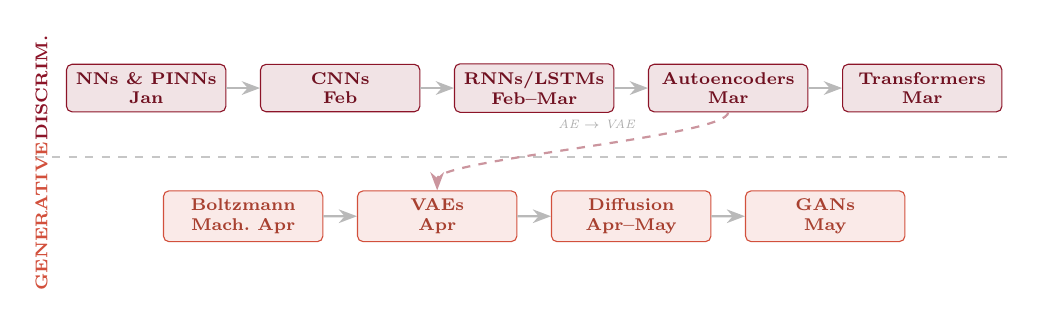
\begin{tikzpicture}[
  box/.style={rectangle, rounded corners=2pt, minimum width=2.3cm,
              minimum height=0.58cm, align=center,
              font=\scriptsize\bfseries},
  discbox/.style={box, fill=mlred!12, draw=mlred, text=mlred!80!black},
  genbox/.style={box, fill=mlcoral!12, draw=mlcoral, text=mlcoral!80!black},
  arr/.style={-Stealth, thick, gray!55},
  scale=0.88, transform shape
]
\node[discbox] (nn)  at (0,0)     {NNs \& PINNs\\Jan};
\node[discbox] (cnn) at (2.8,0)   {CNNs\\Feb};
\node[discbox] (rnn) at (5.6,0)   {RNNs/LSTMs\\Feb--Mar};
\node[discbox] (ae)  at (8.4,0)   {Autoencoders\\Mar};
\node[discbox] (tr)  at (11.2,0)  {Transformers\\Mar};
\draw[arr] (nn)--(cnn); \draw[arr] (cnn)--(rnn);
\draw[arr] (rnn)--(ae); \draw[arr] (ae)--(tr);
\node[left, font=\scriptsize\bfseries, text=mlred] at (-1.3,0)
  {\rotatebox{90}{DISCRIM.}};
\draw[dashed, thick, gray!45] (-1.6,-1.0) -- (12.5,-1.0);
\node[genbox] (bm)   at (1.4,-1.85) {Boltzmann\\Mach.\ Apr};
\node[genbox] (vae)  at (4.2,-1.85) {VAEs\\Apr};
\node[genbox] (diff) at (7.0,-1.85) {Diffusion\\Apr--May};
\node[genbox] (gan)  at (9.8,-1.85) {GANs\\May};
\draw[arr] (bm)--(vae); \draw[arr] (vae)--(diff);
\draw[arr] (diff)--(gan);
\node[left, font=\scriptsize\bfseries, text=mlcoral] at (-1.3,-1.85)
  {\rotatebox{90}{GENERATIVE}};
\draw[arr, dashed, mlred!45] (ae.south)
  .. controls +(0,-0.35) and +(0,0.45) .. (vae.north);
\node[font=\tiny\itshape, text=gray!65] at (6.5,-0.52) {AE $\to$ VAE};
\end{tikzpicture}
\end{center}
\end{frame}

% ============================================================
%  PART I — DISCRIMINATIVE METHODS
% ============================================================
\begin{frame}[plain]
  \begin{center}
    \vspace{1.6cm}
    {\Huge\bfseries\color{mlred} Part I}\\[0.5em]
    {\Large\color{mldark} Discriminative Deep Learning}\\[0.35em]
    {\normalsize\color{gray} January -- March}
  \end{center}
\end{frame}

% ---- Week 1 ------------------------------------------------
\begin{frame}{{\color{mlgold}\textbf{Week 1 (Jan 19--23)}\;---\;Course Introduction \& NN Basics}}
  \begin{columns}[T]
    \column{0.54\textwidth}
      \begin{block}{Mathematics of Deep Learning}
        \begin{itemize}\itemsep1pt
          \item Neurons, layers, activation functions
          \item Forward pass (compact form):\\
                $\bm{a}^{(l)} = \sigma\!\bigl(\bm{W}^{(l)}\bm{a}^{(l-1)}+\bm{b}^{(l)}\bigr)$
          \item Loss functions and optimisation
          \item Backpropagation: chain rule
          \item Writing a NN from scratch
        \end{itemize}
      \end{block}
    \column{0.43\textwidth}
      \begin{block}{Overview \& Projects}
        \begin{itemize}\itemsep2pt
          \item Course structure and themes
          \item Deep learning in the physical sciences: survey
          \item Discussion of project topics
          \item Tools: PyTorch / JAX
        \end{itemize}
      \end{block}
      \vspace{3pt}
      \begin{alertblock}{Goal}
        Build a NN from first principles
        before using high-level frameworks.
      \end{alertblock}
  \end{columns}
\end{frame}

% ---- Week 2 ------------------------------------------------
\begin{frame}{{\color{mlgold}\textbf{Week 2 (Jan 26--30)}\;---\;NNs for Differential Equations}}
  \begin{columns}[T]
    \column{0.54\textwidth}
      \begin{block}{Deep Learning Mathematics (cont.)}
        \begin{itemize}\itemsep1pt
          \item Optimisers: SGD, Adam, RMSProp
          \item Regularisation: dropout, batch norm
          \item Universal approximation theorem
          \item Practical NN coding session
        \end{itemize}
      \end{block}
    \column{0.43\textwidth}
      \begin{block}{Solving ODEs / PDEs}
        \begin{itemize}\itemsep1pt
          \item NNs as mesh-free function approximators
          \item Loss encodes boundary conditions
          \item Advantages and limitations
          \item Code examples: simple ODEs
        \end{itemize}
      \end{block}
  \end{columns}
  \vspace{4pt}
  \begin{exampleblock}{Bridge to the Physical Sciences}
    NNs that solve differential equations are one of the most direct
    applications of deep learning to the physical sciences.
  \end{exampleblock}
\end{frame}

% ---- Week 3 ------------------------------------------------
\begin{frame}{{\color{mlgold}\textbf{Week 3 (Feb 2--6)}\;---\;Physics-Informed Neural Networks (PINNs)}}
  \begin{columns}[T]
    \column{0.54\textwidth}
      \begin{block}{PINNs: Key Idea}
        Embed the PDE directly into the loss function:
        \[
          \mathcal{L} = \mathcal{L}_{\rm PDE} + \lambda\,\mathcal{L}_{\rm BC}
        \]
        \begin{itemize}\itemsep1pt
          \item Automatic differentiation for residuals
          \item Hard vs.\ soft BC enforcement
          \item Schr\"{o}dinger, heat, Poisson as examples
        \end{itemize}
      \end{block}
    \column{0.43\textwidth}
      \begin{block}{Implementation \& Results}
        \begin{itemize}\itemsep1pt
          \item Network architecture choices
          \item Collocation point sampling
          \item Training strategies
          \item Benchmarking vs.\ classical solvers
          \item Limitations of PINNs
        \end{itemize}
      \end{block}
  \end{columns}
\end{frame}

% ---- Weeks 4--5 --------------------------------------------
\begin{frame}{{\color{mlgold}\textbf{Weeks 4--5 (Feb 9--20)}\;---\;Convolutional Neural Networks}}
  \begin{columns}[T]
    \column{0.48\textwidth}
      \begin{block}{Week 4: CNN Mathematics}
        \begin{itemize}\itemsep1pt
          \item Discrete convolution and cross-correlation
          \item Filters, feature maps, receptive fields
          \item Pooling: max, average, global
          \item Parameter sharing, equivariance
          \item Backprop through conv layers
        \end{itemize}
      \end{block}
    \column{0.48\textwidth}
      \begin{block}{Week 5: Architectures \& Codes}
        \begin{itemize}\itemsep1pt
          \item Classic architectures: LeNet, ResNet, U-Net
          \item Skip connections and residual learning
          \item CNNs for physics: images, fields, spectra
          \item Code walkthrough and tuning
        \end{itemize}
      \end{block}
  \end{columns}
  \vspace{4pt}
  \begin{exampleblock}{Applications}
    CNNs excel at identifying spatial patterns in simulation
    output, detector images, and lattice field configurations.
  \end{exampleblock}
\end{frame}

% ---- Weeks 6--7 --------------------------------------------
\begin{frame}{{\color{mlgold}\textbf{Weeks 6--7 (Feb 23 -- Mar 6)}\;---\;Recurrent Neural Networks \& LSTMs}}
  \begin{columns}[T]
    \column{0.54\textwidth}
      \begin{block}{Recurrent Neural Networks}
        \begin{itemize}\itemsep1pt
          \item Sequential data: time series, trajectories
          \item Vanilla RNN hidden-state update:\\
                $\bm{h}_t = \tanh(\bm{W}_{hh}\bm{h}_{t-1}
                            +\bm{W}_{xh}\bm{x}_t+\bm{b})$
          \item Backpropagation through time (BPTT)
          \item Vanishing / exploding gradients
        \end{itemize}
      \end{block}
    \column{0.43\textwidth}
      \begin{block}{Long Short-Term Memory}
        \begin{itemize}\itemsep1pt
          \item LSTM gates: forget, input, output
          \item Cell state as long-range memory
          \item GRUs as a lighter alternative
          \item Applications:\\
                molecular dynamics,\\
                time-series forecasting
        \end{itemize}
      \end{block}
  \end{columns}
\end{frame}

% ---- Weeks 8--9 --------------------------------------------
\begin{frame}{{\color{mlgold}\textbf{Weeks 8--9 (Mar 9--20)}\;---\;Autoencoders \& Dimensionality Reduction}}
  \begin{columns}[T]
    \column{0.48\textwidth}
      \begin{block}{Autoencoders}
        Encoder--decoder: $\bm{x}\to\bm{z}\to\hat{\bm{x}}$
        \begin{itemize}\itemsep1pt
          \item Bottleneck latent space $\bm{z}$
          \item Reconstruction loss $\|\bm{x}-\hat{\bm{x}}\|^2$
          \item Denoising autoencoders
          \item Convolutional AE architectures
        \end{itemize}
      \end{block}
    \column{0.48\textwidth}
      \begin{block}{Links to PCA \& Implementations}
        \begin{itemize}\itemsep1pt
          \item Linear AE $\equiv$ PCA (exactly)
          \item Kernel PCA, nonlinear extensions
          \item Latent space visualisation
          \item Applications: order parameters,
                phase classification, compression
          \item Code walkthrough (Week 9)
        \end{itemize}
      \end{block}
  \end{columns}
\end{frame}

% ---- Week 10 -----------------------------------------------
\begin{frame}{{\color{mlgold}\textbf{Week 10 (Mar 23--27)}\;---\;Transformers \& Part I Summary}}
  \begin{columns}[T]
    \column{0.54\textwidth}
      \begin{block}{The Transformer Architecture}
        Self-attention: $\mathrm{Att}(Q,K,V)
          =\mathrm{softmax}\!\bigl(QK^\top/\!\sqrt{d_k}\bigr)V$
        \begin{itemize}\itemsep1pt
          \item Multi-head attention
          \item Positional encoding
          \item Encoder / decoder stacks
          \item Applications: quantum chemistry, PDEs and many other
        \end{itemize}
      \end{block}
    \column{0.43\textwidth}
      \begin{alertblock}{Part I Summary}
        \textbf{Five discriminative families:}
        \begin{enumerate}\itemsep1pt
          \item Feed-forward NNs \& PINNs
          \item CNNs
          \item RNNs / LSTMs
          \item Autoencoders
          \item Transformers
        \end{enumerate}
        Each tackles a distinct structural
        challenge in  data from the physical sciences.
      \end{alertblock}
  \end{columns}
\end{frame}

% ============================================================
%  PART II — GENERATIVE METHODS
% ============================================================
\begin{frame}[plain]
  \begin{center}
    \vspace{1.6cm}
    {\Huge\bfseries\color{mlcoral} Part II}\\[0.5em]
    {\Large\color{mldark} Generative Deep Learning}\\[0.35em]
    {\normalsize\color{gray} April -- May}
  \end{center}
\end{frame}

% ---- Week 11 -----------------------------------------------
\begin{frame}{{\color{mlgold}\textbf{Week 11 (Apr 6--10)}\;---\;Generative Models \& Boltzmann Machines}}
  \begin{columns}[T]
    \column{0.54\textwidth}
      \begin{block}{What Are Generative Models?}
        \begin{itemize}\itemsep1pt
          \item Goal: learn $p_\theta(\bm{x})\approx p_{\rm data}(\bm{x})$
          \item Explicit vs.\ implicit density estimation
          \item Energy-based models:
                $p_\theta(\bm{x}) = e^{-E_\theta(\bm{x})}/Z(\theta)$
          \item Markov Chain Monte Carlo recap
          \item Gibbs sampling
        \end{itemize}
      \end{block}
    \column{0.43\textwidth}
      \begin{block}{Boltzmann Machines}
        \begin{itemize}\itemsep1pt
          \item Restricted BM: visible \& hidden units
          \item Contrastive Divergence (CD-$k$)
          \item Persistent CD and variants
          \item Deep Boltzmann Machines
          \item Statistical mechanics analogy
        \end{itemize}
      \end{block}
  \end{columns}
\end{frame}

% ---- Week 12 -----------------------------------------------
\begin{frame}{{\color{mlgold}\textbf{Week 12 (Apr 13--17)}\;---\;Energy-Based Models \& BM Codes}}
  \begin{columns}[T]
    \column{0.54\textwidth}
      \begin{block}{Energy-Based Models (Deeper Dive)}
        \begin{itemize}\itemsep1pt
          \item Score matching and noise contrastive estimation
          \item Contrastive Divergence revisited
          \item Expressivity of energy functions
          \item Links to partition functions in statistical physics
          \item Training instabilities and remedies
        \end{itemize}
      \end{block}
    \column{0.43\textwidth}
      \begin{block}{Boltzmann Machine Codes}
        \begin{itemize}\itemsep1pt
          \item Implementing an RBM from scratch
          \item Sampling via Gibbs chains
          \item Visualising learned features
          \item Wave-function ansatz application
          \item Benchmarks and diagnostics
        \end{itemize}
      \end{block}
  \end{columns}
  \vspace{3pt}
  \begin{exampleblock}{Highlight}
    RBMs have been used as variational ans\"{a}tze for quantum
    many-body ground states --- a direct link to quantum computing.
  \end{exampleblock}
\end{frame}

% ---- Week 13 -----------------------------------------------
\begin{frame}{{\color{mlgold}\textbf{Week 13 (Apr 20--24)}\;---\;Variational Autoencoders (VAEs)}}
  \begin{columns}[T]
    \column{0.54\textwidth}
      \begin{block}{VAE: Probabilistic Autoencoders}
        \begin{itemize}\itemsep1pt
          \item Latent variable model:
                $p(\bm{x})=\int p(\bm{x}|\bm{z})p(\bm{z})\,\mathrm{d}\bm{z}$
          \item ELBO objective:
                $\mathcal{L} = \mathbb{E}_{q}[\log p(\bm{x}|\bm{z})]
                              - D_{\rm KL}(q\|p)$
          \item Reparameterisation trick
          \item Encoder $\to (\bm\mu,\bm\sigma)$;
                Decoder $\to\hat{\bm{x}}$
        \end{itemize}
      \end{block}
    \column{0.43\textwidth}
      \begin{block}{VAE vs.\ Standard AE}
        \begin{itemize}\itemsep1pt
          \item Structured, continuous latent space
          \item Sample: $\bm{z}\sim\mathcal{N}(0,I)$
          \item Disentanglement ($\beta$-VAE)
          \item Applications:\\
                molecular generation,\\
                anomaly detection,\\
                data interpolation
        \end{itemize}
      \end{block}
  \end{columns}
\end{frame}

% ---- Week 14 -----------------------------------------------
\begin{frame}{{\color{mlgold}\textbf{Week 14 (Apr 27 -- May 1)}\;---\;Diffusion Models}}
  \begin{columns}[T]
    \column{0.54\textwidth}
      \begin{block}{Denoising Diffusion Probabilistic Models}
        \begin{itemize}\itemsep1pt
          \item Forward: add Gaussian noise gradually\\
                $q(\bm{x}_t|\bm{x}_{t-1})
                 =\mathcal{N}(\sqrt{1-\beta_t}\,\bm{x}_{t-1},\beta_t\bm{I})$
          \item Reverse: learn to denoise step-by-step
          \item Score matching and Langevin dynamics
          \item Noise schedules: linear, cosine
          \item Link to stochastic differential equations
        \end{itemize}
      \end{block}
    \column{0.43\textwidth}
      \begin{block}{Why Diffusion Models?}
        \begin{itemize}\itemsep1pt
          \item State-of-the-art sample quality
          \item Stable training vs.\ GANs
          \item Conditional generation
          \item Applications:\\
                molecular structure,\\
                protein folding,\\
                lattice field theory
        \end{itemize}
      \end{block}
  \end{columns}
\end{frame}

% ---- Week 15 -----------------------------------------------
\begin{frame}{{\color{mlgold}\textbf{Week 15 (May 4--8)}\;---\;Diffusion Models (cont.) \& GANs}}
  \begin{columns}[T]
    \column{0.48\textwidth}
      \begin{block}{Diffusion: Codes \& Implementations}
        \begin{itemize}\itemsep1pt
          \item Implementing DDPM from scratch
          \item U-Net backbone for the denoiser
          \item Training loop and ELBO loss
          \item Sampling procedures
          \item Classifier-free guidance
        \end{itemize}
      \end{block}
    \column{0.48\textwidth}
      \begin{block}{Generative Adversarial Networks}
        {\small Minimax: $\min_G\max_D\;
          \mathbb{E}[\log D(\bm{x})]
         +\mathbb{E}[\log(1{-}D(G(\bm{z})))]$}
        \begin{itemize}\itemsep1pt
          \item Training dynamics and mode collapse
          \item Wasserstein GAN (WGAN)
          \item Conditional GANs (cGAN)
        \end{itemize}
      \end{block}
  \end{columns}
\end{frame}

% ---- Week 16 (final) ----------------------------------------
\begin{frame}{{\color{mlgold}\textbf{Week 16 (May 18--22)}\;---\;GANs (cont.) \& Project Discussions}}
  \begin{columns}[T]
    \column{0.54\textwidth}
      \begin{block}{Advanced GAN Topics}
        \begin{itemize}\itemsep1pt
          \item Architectures: DCGAN, StyleGAN, CycleGAN
          \item Evaluation: FID, IS, precision/recall
          \item GANs: fast simulation,
                inverse problems, lattice QCD
          \item GANs vs.\ diffusion: trade-offs
        \end{itemize}
      \end{block}
    \column{0.43\textwidth}
      \begin{alertblock}{Project Presentations}
        Applications across the curriculum:
        \begin{itemize}\itemsep1pt
          \item PINNs for PDEs
          \item CNNs for detector data
          \item RBMs as wave-function ans\"{a}tze
          \item VAEs for molecular design
          \item Diffusion / GANs for fast simulation
        \end{itemize}
      \end{alertblock}
  \end{columns}
\end{frame}

% ---- Road map table: Part I ---------------------------------
\begin{frame}{Weekly Road Map --- Part I: Discriminative Methods}
\begin{center}
\scriptsize
\renewcommand{\arraystretch}{1.30}
\begin{tabular}{@{}lll p{7.8cm}@{}}
  \toprule
  \textbf{Week} & \textbf{Dates} & \textbf{Part} & \textbf{Topics} \\
  \midrule
  1    & Jan 19--23    & \disctext{Discriminative}
       & Course intro, NN basics, backpropagation, project discussion \\
  2    & Jan 26--30    & \disctext{Discriminative}
       & NN codes, optimisers, regularisation, solving ODEs with NNs \\
  3    & Feb 2--6      & \disctext{Discriminative}
       & Physics-Informed Neural Networks (PINNs) \\
  4--5 & Feb 9--20     & \disctext{Discriminative}
       & Convolutional NNs: mathematics, architectures, codes \\
  6--7 & Feb 23--Mar 6 & \disctext{Discriminative}
       & Recurrent NNs, LSTMs, backprop through time \\
  8--9 & Mar 9--20     & \disctext{Discriminative}
       & Autoencoders, PCA, latent space, implementations \\
  10   & Mar 23--27    & \disctext{Discriminative}
       & Transformers, self-attention, Part I summary \\
  \bottomrule
\end{tabular}
\end{center}
\end{frame}

% ---- Road map table: Part II --------------------------------
\begin{frame}{Weekly Road Map --- Part II: Generative Methods}
\begin{center}
\scriptsize
\renewcommand{\arraystretch}{1.30}
\begin{tabular}{@{}lll p{7.8cm}@{}}
  \toprule
  \textbf{Week} & \textbf{Dates} & \textbf{Part} & \textbf{Topics} \\
  \midrule
  11   & Apr 6--10     & \gentext{Generative}
       & Generative models overview, Boltzmann machines, MCMC, Gibbs \\
  12   & Apr 13--17    & \gentext{Generative}
       & Energy-based models, RBM codes, wave-function ansatz \\
  13   & Apr 20--24    & \gentext{Generative}
       & Variational autoencoders (VAEs), ELBO, reparameterisation \\
  14   & Apr 27--May 1 & \gentext{Generative}
       & Diffusion models: forward/reverse process, score matching \\
  15   & May 4--8      & \gentext{Generative}
       & Diffusion codes (DDPM), GANs: minimax, WGAN, cGAN \\
  16   & May 18--22    & \gentext{Generative}
       & Advanced GANs, evaluation metrics, project presentations \\
  \bottomrule
\end{tabular}
\end{center}
\end{frame}

% ---- Closing -----------------------------------------------
\begin{frame}{What You Will Know at the End}
  \begin{columns}[T]
    \column{0.48\textwidth}
      \begin{block}{Discriminative Skills}
        \begin{itemize}\itemsep2pt
          \item Derive and implement backpropagation
          \item Build NNs, CNNs, RNNs, and PINNs
          \item Solve ODEs and PDEs with neural networks
          \item Design autoencoders for data reduction
          \item Understand attention and transformers
        \end{itemize}
      \end{block}
    \column{0.48\textwidth}
      \begin{block}{Generative Skills}
        \begin{itemize}\itemsep2pt
          \item Train Boltzmann machines and sample from them
          \item Derive and implement the VAE ELBO
          \item Implement denoising diffusion models
          \item Train and stabilise GANs
          \item Apply generative models to problems in the physical sciences
        \end{itemize}
      \end{block}
  \end{columns}
  \vspace{5pt}
  \begin{alertblock}{Overarching Goal}
    Build both the \textbf{mathematical foundations} and the
    \textbf{practical implementation skills} to apply state-of-the-art
    deep learning methods to open problems in the physical sciences.
  \end{alertblock}
\end{frame}

\end{document}
